\chapter{Introduction}\label{C:intro}

Test suites are an important part in every major software project \cite{jeffrey2005test}. They check a specified set of behaviours are met by a software program. Meeting the behaviours increase the confidence in the program, but as a consequence, a large number of tests need to be executed and may take up to several hours to run.

Test cases are added to the test suite throughout the project, often when a piece of code is altered, new code is developed or a bug gets fixed \cite{issuetrack,whentotest}. With tests being added throughout, it is desirable to ensure that any new test case is not replicating the behaviour of any of the previous. Even with careful planning, it is difficult to avoid redundant test cases. The goals of the project are to create a tool to identify these test cases within a test suite. After the tools creation, its capability to identify redundant tests are explored through experiments.


The execution of a test case leaves a trail of data. This trail contains information ranging from low level to high level run time data. A low level example would be machine code while a high level could be the method execution data. A variety of previous research \cite{wong1995effect, wong1999test, rothermel1998empirical, rothermel2002empirical,koochakzadeh2009test,zhang2011empirical,li2008static} discusses using some of this information to identify redundant test cases. The papers identify redundant tests using statement coverage while the majority examine benchmarks with under 200 test cases. For benchmarks with a large number of test cases storing every statement execution could be costly, therefore our project investigates using method execution data to identify redundant test cases. One of the issues that previous studies reported was a high level of false positives. Method execution data gives different ways to explore this issue which are explored further on. 

The tool developed can analyse method execution details, known as \textit{test spectra}, to determine the level of redundancy between two tests. This analysis can identify potentially redundant test cases. Figure \ref{fig:spectra} shows a basic visualisation of the idea. The spectra are three different tests where colours represent method executions. Intuitively, it is clear that Test 1 is different from Tests 2 and 3 as the method executions is different between them however, there are similarities between Tests 2 and 3 which could identify some level of redundancy between the test cases. 

\begin{figure}[h]
\centering
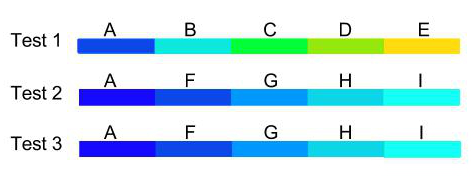
\includegraphics[width=6cm,height=3cm]{spectra.png}
\caption{A spectra where each colour represents different method execution details. We see similarities between Tests 2 and 3. In contrast, Test 1 is different from 2 and 3. }
\label{fig:spectra}
\end{figure}

Once the tests are identified as being redundant, they may be removed, however it is important to understand the dangers of removing test cases. Unless two test cases are exactly the same, it is difficult to guarantee whether one is redundant, even if one subsumes another. This creates the need to be able to use different techniques, dependent on the benchmark. To expand on the goal of the project, the developed tool should give developers different approaches for identifying redundant test cases. The tool should allow a developer to configure different analysis metrics and view the results. Overall, the tool will be useful for gaining an overview and understanding of the condition of the test suite, allowing for manual inspection to determine if the identified redundant tests should be removed.

Another potential use case of the tool is to redistribute the test cases. This can be achieved by splitting the non redundant tests into another test suite and running this suite in place of the original. The original test suite may be run over night when no development is occurring. This separation of tests based on redundancy allows for a testing process, for example regression testing, to occur in a timely fashion while ensuring the original bug finding ability is retained. This is applicable to David Pearce, who is currently writing a language called Whiley. The language contains an extended static checking tool to eliminate run time exceptions through formal verification techniques. In the main compiler module alone, there are roughly 20,000 tests. Relocating some these tests into another suite would allow him to increase development speed. This is due to the reduction in the time taken to run his test suite. This reduction also gives David incentive to execute his suite more often. This increase in frequency allows him to trace back bugs to code changes easier and reduces his time spent debugging. 

The contributions of the project is split into two parts: 

\begin{itemize}
\item Create a tool for identifying redundant test cases
\item Analyse different strategies for identifying redundant test cases through experimenting on realistic benchmarks
\end{itemize}

\section{Outline}

The report is structured as follows. Chapter 2 discusses previous research in this area of interest. It also examines background information and explores the concepts needed to understand the following chapters. The design and implementation of the tool is then examined in Chapter 3. Chapter 4 investigates the different techniques then conducts and discusses some experiments. Finally, Chapter 5 concludes the report and identifies future work.